% ----------------------------------------------------------
% Chapter 1
% ----------------------------------------------------------
\chapter{Introduction}
% ----------------------------------------------------------

Concurrency is an attribute of any system that allows multiple components to perform operations at the same time. The understanding of this property is essential in modern programming because major areas, such as distributed and real-time systems, rely on this concept to work properly. As a result, the variety of applications enabled by the concurrency feature is broad: aircraft and industrial control systems, routing algorithms, peer-to-peer networks, client-server applications and parallel computation, to name a few.

Since concurrent systems may have parts that execute in parallel, the combination of ways in which these parts can interact raises the complexity in designing such systems. Phenomena like deadlock, livelock, nondeterminism and race condition can emerge from these interactions, so these issues must be addressed in order to avoid undesired behavior. Typically, testing cannot provide enough evidence to guarantee properties such as deadlock freedom, divergence freedom and determinism for a given system.

That being said, CSP (a theory for Communicating Sequential Processes) introduces a convenient notation that allows systems to be described in a clear and accurate way. More than that, it has an underlying theory that enables designs to be analysed and proven correct with respect to desired properties. The FDR (Failures-Divergence Refinement) tool is a model checker for CSP responsible for making this process algebra a practical tool for specification, analysis and verification of systems. System analysis is achieved by allowing the user to make assertions about processes and then exploring every possible behavior, if necessary, to check the truthfulness of the assertions made.

Although it is undeniable that FDR is a useful tool in the analysis of systems described in CSP, it has a limitation common to standard model checkers in general: the state explosion problem. An alternative way for deciding whether a system meets its specification is by proof development. Examples of this different approach are CSP-Prover and Isabelle/UTP, both frameworks based on the theorem prover Isabelle. Nevertheless, to the best of our knowledge, there is not a theory for CSP in the Coq proof assistant yet. Considering that, the main research question of this work is the following: how could we develop a theory of CSP in Coq, exploiting the main advantages of this proof assistant?

% ---
\section{Objectives}
% ---

The main objective (MO) of this work is to define in Coq a theory for concurrent systems, based on a limited scope of the process algebra CSP. This objective is unfolded into the following specific objectives (SO):

\begin{itemize}  
	\item SO1: study CSP and frameworks based on this process algebra. 
	\item SO2: define a syntax for CSP in Coq, based on a restricted version of the CSP\textsubscript{M} language (machine readable language for CSP). 
	\item SO3: provide support for the LTS-based (Labelled Transition System) representation, considering the Structural Operational Semantics (SOS) of CSP.
	\item SO4: make use of the QuickChick tool to search for counterexamples of the traces refinement relation.
\end{itemize}

% ---
\section{An overview of CSP\textsubscript{Coq}}
% ---

\begin{coqdoccode}
	\coqdocnoindent
	\coqdockw{Require} \coqdockw{Import} \coqdocvar{CSP.lts}.\coqdoceol
	\coqdocnoindent
	\coqdockw{Require} \coqdockw{Import} \coqdocvar{CSP.semantics\_sos}.\coqdoceol
	\coqdocnoindent
	\coqdockw{Require} \coqdockw{Import} \coqdocvar{CSP.semantics\_trace}.\coqdoceol
	\coqdocnoindent
	\coqdockw{Require} \coqdockw{Import} \coqdocvar{CSP.syntax}.\coqdoceol
	\coqdocnoindent
	\coqdockw{Require} \coqdockw{Import} \coqdocvar{Lists.List}.\coqdoceol
	\coqdocnoindent
	\coqdockw{Require} \coqdockw{Import} \coqdocvar{Lists.ListSet}.\coqdoceol
	\coqdocnoindent
	\coqdockw{Require} \coqdockw{Import} \coqdocvar{Strings.String}.\coqdoceol
	\coqdocnoindent
	\coqdockw{Import} \coqdocvar{ListNotations}.\coqdoceol
	\coqdocemptyline
	\coqdocnoindent
	\coqdockw{Local Open} \coqdockw{Scope} \coqdocvar{string}.\coqdoceol
	\coqdocemptyline
	\coqdocnoindent
	\coqdockw{Definition} \coqdocvar{example} : \coqdocvar{specification}.\coqdoceol
	\coqdocnoindent
	\coqdockw{Proof}.\coqdoceol
	\coqdocindent{1.00em}
	\coqdocvar{solve\_spec\_ctx\_rules} (\coqdoceol
	\coqdocindent{2.00em}
	\coqdocvar{Build\_Spec}\coqdoceol
	\coqdocindent{2.00em}
	[\coqdoceol
	\coqdocindent{3.00em}
	\coqdocvar{Channel} \{\{"start", "ev1", "ev2", "ev3", "end"\}\}\coqdoceol
	\coqdocindent{2.00em}
	]\coqdoceol
	\coqdocindent{2.00em}
	[\coqdoceol
	\coqdocindent{3.00em}
	"P" ::= "start" --> ("ev1" --> \coqdocvar{SKIP} [] "ev2" --> \coqdocvar{SKIP}) ;; "end" --> \coqdocvar{ProcRef} "P"\coqdoceol
	\coqdocindent{3.00em}
	; "Q" ::= "start" --> "ev3" --> "end" --> \coqdocvar{ProcRef} "Q"\coqdoceol
	\coqdocindent{3.00em}
	; "R" ::= \coqdocvar{ProcRef} "P" [| \{\{"start", "end"\}\} |] \coqdocvar{ProcRef} "Q"\coqdoceol
	\coqdocindent{2.00em}
	]\coqdoceol
	\coqdocindent{1.00em}
	).\coqdoceol
	\coqdocnoindent
	\coqdockw{Defined}.\coqdoceol
	\coqdocemptyline
	\coqdocnoindent
	\coqdockw{Compute} \coqdocvar{generate\_dot} (\coqdocvar{compute\_ltsR} \coqdocvar{example} "R" 100).\coqdoceol
\end{coqdoccode}

\begin{figure}[htb]
	\caption{\label{lts-example}The "R" process LTS.}
	\begin{center}
		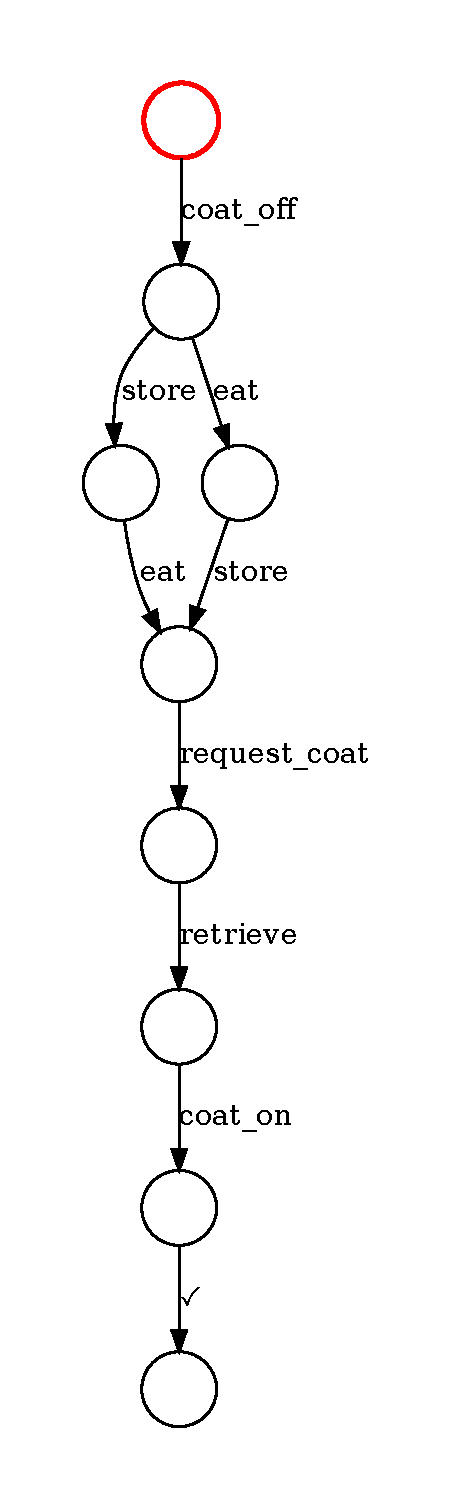
\includegraphics[scale=0.75]{images/LTS.pdf}
	\end{center}
	\legend{Source: }
\end{figure}

% ---
\section{Main contributions}
% ---

The main contributions of this work are the following:

\begin{itemize}
	\item abstract and concrete syntax
	\item structured operational semantics
	\item labelled transition systems (inductive + functional)
	\item proof of correctness of this functional definition
	\item traces (inductive + functional)
	\item proof of correctness of this functional definition
	\item traces refinement (formal definition)
	\item refinement verification using QuickChick
\end{itemize}

% ---
\section{Document structure}
% ---

Apart from this introductory chapter, in which we discuss about the motivation behind this work and its main objective, and also take a quick look at an example that illustrates what can be done using the framework developed, this monograph contains three more chapters. The content of these chapters are detailed bellow:
\begin{description}
	\item [Chapter 2] Discusses fundamental concepts such as CSP theory, SOS approach, trace refinement and LTS representation. Moreover, this chapter introduces the Coq proof assistant and its functional language Gallina, along with an introduction to proof development (tactics) and the Ltac language inside this tool, which gives support for developing tactic macros.
	\item [Chapter 3] Provides an in-depth look at the implementation of CSP\textsubscript{Coq}, including its abstract and concrete syntax, and language semantics. Furthermore, the LTS process representation support, using the GraphViz software, is also detailed in this chapter.
	\item [Chapter 4] Concludes this monograph by presenting a comparison between the infrastructure described in this work and other interactive theorem provers based on CSP. It also addresses possible topics for future work.
\end{description}